\subsection{Enumeration, Counting, and Random Generation of Ladder Lotteries}

In this paper, the authors consider the problem of enumeration, counting and 
random generation of ladder-lotteries with $N$ lines and $B$ bars \cite{A6}. 
It is important to note that the authors considered both optimal and 
non-optimal ladders for this paper. Nonetheless, the paper is still fruitful 
for its modelling of the probelems and insights into ladder-lotteries.
The authors use  the line-based encoding, $LC_{L}$ for the representation of ladders 
that was discussed in the review of \textbf{Coding Ladder Lotteries}.

%%Section for enumeration
\subsubsection{Enumeration}
The authors denote a set of ladder lotteries with $N$ lines and 
$B$ bars as $S_{N,B}$. The problem is how to enumerate all the 
ladders in $S_{N,B}$ \cite{A6}. The authors use a \emph{forest structure}
to model the problem. A \emph{forest structure} is a set of trees 
such that each tree in the forest is dijoint union with every other 
tree in the forest. Consider $S_{N,B}$ to be a tree in a forest.
That is to say, a union disjoint subset of all ladders with $N$
lines and $B$ bars. Then $F_{N,B}$, or the forest of all $S_{N,B}s$,
is the set of all ladders with $N$ lines and $B$ bars \cite{A6}. For an example 
of a forest for $F_{3,2}$ refer to Fig. \ref{fig:forest3,2}\par %figure number.

The authors create $F_{N,R}$ by defining a removal sequennce for 
each $LC_{L}$ \cite{A6}. Each ladder, $L$, in 
$F_{N,R}$ is a leaf node. By removing the second last bit of $LC_{L}$ the result 
is $P(LC_{L})$ and the resulting substructure is some \emph{sub-ladder}, $P(L)$, which 
is an incomplete ladder containing unmatched endpoints of bars or a missining line \cite{A6}. For example, 
given $LC_{L}=10100$, $P(LC_{L})=1010$. Notice how the second last bit was removed. 
By removing the second last bit from $P(LC_{L})$ we get $P(P(LC_{L}))$ and $P(P(L))$ respectively.
The removal sequence is repeated until the sub-ladder consists of two lines with $0$ endpoints
attached to line $2$ and $0$ to $R$ left endpoints are attached to line $1$. There are $R+1$
terminating sub-ladders, i.e., roots of trees in $F_{N, R}$.The removal sequence is uniqe for each ladder in $F_{N,R}$ is unique.\par
\begin{figure}[!htp]
    \begin{center}
    \begin{minipage}{.8\textwidth}
        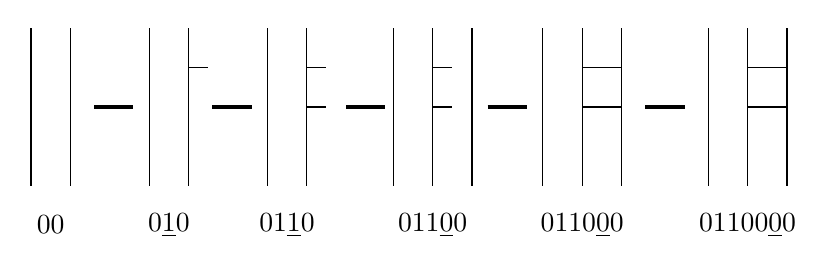
\begin{tikzpicture}
            \draw(0, 0) to (0, 2);
            \draw(0.5, 0) to (0.5, 2);
                \node at(0.25, -0.5){00};

            %%branch
            \draw[line width=0.5mm] (0.8, 1) to (1.3, 1);

            \draw(1.5, 0) to (1.5, 2);
                \draw(2, 1.5) to (2.25, 1.5);
            \draw(2, 0) to (2, 2);
                \node at (1.75, -0.5){0\underline{1}0};
    
            %%branch
            \draw[line width=0.5mm] (2.3, 1) to (2.8, 1);
            
            \draw(3, 0) to (3, 2);
            \draw(3.5, 0) to (3.5, 2);
                 \draw(3.5, 1.5) to (3.75, 1.5);
                 \draw(3.5, 1) to (3.75, 1);
                \node at (3.25, -0.5){01\underline{1}0};
            
            \draw[line width=0.5mm] (4, 1) to (4.5, 1);

            \draw(4.6, 0) to (4.6, 2);
            \draw(5.1, 0) to (5.1, 2);
            \draw(5.6, 0) to (5.6, 2);
                 \draw(5.1, 1.5) to (5.35, 1.5);
                 \draw(5.1, 1) to (5.35, 1);
                \node at (5.1, -0.5){011\underline{0}0};


            \draw[line width=0.5mm](5.8, 1) to (6.3, 1);
            \draw(6.5, 0) to (6.5, 2);
            \draw(7, 0) to (7, 2);
            \draw(7.5, 0) to (7.5, 2);
                \draw(7, 1.5) to (7.5, 1.5);
                \draw(7, 1) to (7.5, 1);
                \node at (7, -0.5){0110\underline{0}0};

            \draw[line width=0.5mm](7.8, 1) to (8.3, 1);
            \draw(8.6, 0) to (8.6, 2);
            \draw(9.1, 0) to (9.1, 2);
            \draw(9.6, 0) to (9.6, 2);
                \draw(9.1, 1.5) to (9.6, 1.5);
                \draw(9.1, 1) to (9.6, 1);
                \node at (9.1, -0.5){01100\underline{0}0};

        \end{tikzpicture}
        
    \end{minipage}
    \end{center}
    
    
  

    %%second tree
    \begin{center}
          \begin{minipage}{0.8\textwidth}
            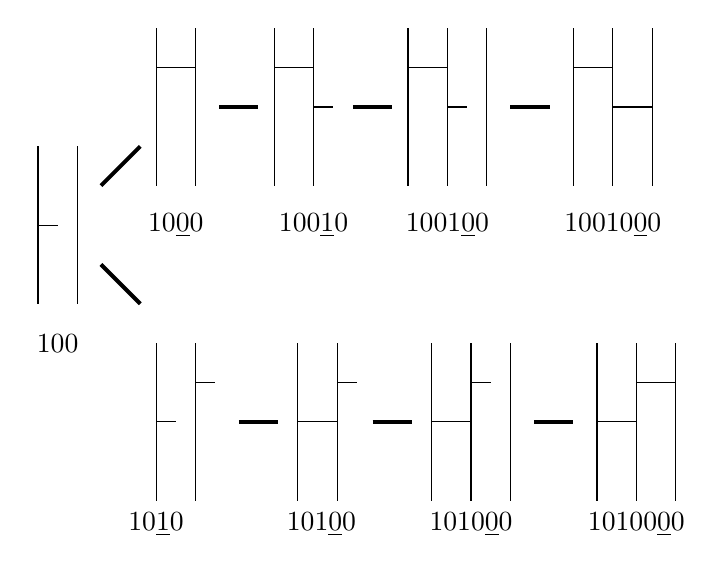
\begin{tikzpicture}
                \draw(0, 0) to (0, 2);
                \draw(0.5, 0) to (0.5, 2);
                    \draw(0, 1) to (0.25, 1);
                    \node at (0.25, -0.5){$100$};
                
                %%upper subtree
                \draw[line width=0.5mm](0.8, 1.5) to (1.3, 2);
                    \draw(1.5, 1.5) to (1.5, 3.5);
                    \draw(2, 1.5) to (2, 3.5);
                        \draw(1.5, 3) to (2, 3);
                        \node at (1.75, 1){$10\underline{0}0$};

                    \draw[line width=0.5mm](2.3, 2.5) to (2.8, 2.5);
                        \draw(3, 1.5) to (3, 3.5);
                            \draw(3, 3) to (3.5,3);
                            \draw(3.5, 2.5) to (3.75, 2.5);
                        \draw(3.5, 1.5) to (3.5, 3.5);
                        \node at (3.5, 1){$100\underline{1}0$};

                    \draw[line width=0.5mm](4, 2.5) to (4.5, 2.5);
                        \draw(4.7,  1.5) to (4.7, 3.5);
                            \draw(4.7, 3) to (5.2, 3);
                            \draw(5.2, 2.5) to (5.45, 2.5);
                        \draw(5.2, 1.5) to (5.2, 3.5);
                        \draw(5.7, 1.5) to (5.7, 3.5);
                        \node at (5.2, 1){$1001\underline{0}0$};

                    \draw[line width=0.5mm](6, 2.5) to (6.5, 2.5);
                        \draw(6.8,  1.5) to (6.8, 3.5);
                            \draw(6.8, 3) to (7.3, 3);
                            \draw(7.3, 2.5) to (7.8, 2.5);
                        \draw(7.3, 1.5) to (7.3, 3.5);
                        \draw(7.8, 1.5) to (7.8, 3.5);
                        \node at (7.3, 1){$10010\underline{0}0$};



                %%lower subtree
                \draw[line width = 0.5mm](0.8, 0.5) to (1.3, 0);
                    \draw (1.5, -0.5) to (1.5, -2.5);
                        \draw(1.5, -1.5) to (1.75, -1.5);
                        \draw(2, -1) to (2.25, -1);
                    \draw(2, -0.5) to (2, -2.5);
                        \node at (1.5, -2.8){$10\underline{1}0$};
                    
                    \draw[line width = 0.5mm](2.55, -1.5) to (3.05, -1.5);

                     \draw (3.3, -0.5) to (3.3, -2.5);
                        \draw(3.3, -1.5) to (3.8, -1.5);
                        \draw(3.8, -1) to (4.05, -1);
                    \draw(3.8, -0.5) to (3.8, -2.5);
                        \node at (3.6, -2.8){$101\underline{0}0$};

                     \draw[line width = 0.5mm](4.25, -1.5) to (4.75, -1.5);

                     \draw (5, -0.5) to (5, -2.5);
                        \draw(5.5, -1) to (5.75, -1);
                        \draw(5, -1.5) to (5.5, -1.5);
                    \draw(5.5, -0.5) to (5.5, -2.5);
                    \draw(6, -0.5) to (6, -2.5);
                        \node at (5.5, -2.8){$1010\underline{0}0$};
                    

                    \draw[line width = 0.5mm](6.3, -1.5) to (6.8, -1.5);
                    \draw (7.1, -0.5) to (7.1, -2.5);
                        \draw(7.1, -1.5) to (7.6, -1.5);
                        \draw(7.6, -1) to (8.1, -1);
                    \draw(7.6, -0.5) to (7.6, -2.5);
                    \draw(8.1, -0.5) to (8.1, -2.5);
                        \node at (7.6, -2.8){$10100\underline{0}0$};
                    

                    
            \end{tikzpicture}
            
        \end{minipage}
    \end{center}


    \begin{center}
        \begin{minipage}{0.8\textwidth}
            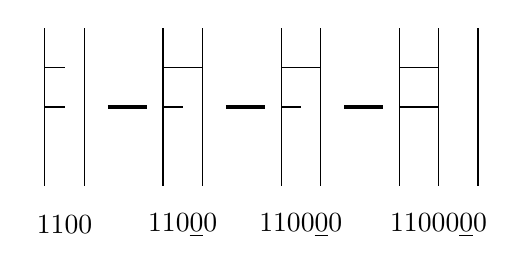
\begin{tikzpicture}%% start pocture
            
            
                \draw(0, 0) to (0, 2);
                    \draw(0, 1.5) to (0.25, 1.5);
                    \draw(0, 1) to (0.25, 1);
                \draw(0.5, 0) to (0.5, 2);
                \node at (0.25, -0.5){$1100$};
            
            
                \draw[line width=0.5mm] (0.8, 1) to (1.3, 1);
                    \draw(1.5, 0) to (1.5, 2);
                        \draw(1.5, 1.5) to (2, 1.5);
                        \draw(1.5, 1) to (1.75, 1);
                    \draw(2, 0) to (2, 2);
                    \node at (1.75, -0.5){$110\underline{0}0$};
            
        
                \draw[line width=0.5mm] (2.3, 1) to (2.8, 1);
                    \draw(3, 0) to (3, 2);
                       \draw(3, 1.5) to (3.5, 1.5);
                       \draw(3, 1) to (3.25, 1);
                   \draw(3.5, 0) to (3.5, 2);
                    \node at (3.25, -0.5){$1100\underline{0}0$};
            
            
                \draw[line width=0.5mm] (3.8, 1) to (4.3, 1);
                    \draw(4.5, 0) to (4.5, 2);
                          \draw(4.5, 1.5) to (5, 1.5);
                          \draw(4.5, 1) to (5, 1);
                      \draw(5, 0) to (5, 2);
                      \draw(5.5, 0) to (5.5, 2);
                          \node at (5, -0.5){$11000\underline{0}0$};
               
            \end{tikzpicture}%%end picture
        \end{minipage}
    \end{center}
    \caption{The forest, $F_{3,2}$ where $3$ is the number of lines and $2$ is the number of bars. All ladders with $3$ lines and $2$ bars are leaf nodes of one of three trees $S_{3,2}$.
    The underlined bits are the inserted second last bit from the parent's line-encoding resulting in the child's line encoding}
    \label{fig:forest3,2}
\end{figure}

%%end enumeratiom section

%%section for counting
\subsubsection{Counting}
The authors provide a method and algorithm to count all ladders 
with $N$ lines and $B$ bars. According to the authors, the enumeration algorithm is 
much slower than the counting algorithm \cite{A6}. The counting algorithm 
works by dividing ladders into four types of sub-ladders.
For sub-ladder, $R$, its type is a tuple $t(n,h,p,q)$ where 
$n$ is the number of lines, $h$ is the number of half bars, 
$p$ is the number of unmatched end-points on line $n-1$ and 
$q$ is the number of unmatched end-points on line $n$. From this 
type there are four sub-divisions of sub-ladders.
\paragraph{ $h < p+q$ or $n<2$}
There are zero ladders because it is impossible for the 
root sub-ladder to have less than two lines. It is also 
impossible for the number of half bars, $h$, to 
be less than the number of detached left end points 
on line $n-1$ plus the number of detached end points on 
line $n$.

%%\subsubsubsection{Case 2: $n=2$ and $h=p$ and $q=0$}
\paragraph{$n=2$ and $h=p$ and $q=0$}
There is only one ladder because the number of half bars 
on the last/$2nd$ line is 0 since $q=0$. Therefore all half bars are on the 
$n-1th$/$1st$ line of the sub-ladder. This is known because 
$h=p$ which means the number of half bars is the same as 
the number of unmatched bars on line $n-1$/$1st$ Hence, the unmacthed 
half bars on the $1st$ line must be connected to the $2nd$ 
line. Once these are all matched the ladder will be complete. 
Thus, there is only one ladder for this case.

%%\subsubsubsection{Case 3: $(n \geq 3$ or $h>p)$ and $q=0$}
\paragraph{$(n \geq 3$ or $h>p)$ and $q=0$}
If this is the case, then there are no endpoints attached to 
line $n$, but the number of half bars is greater than the 
number of enpoints attached to line $n-1$, which means there is 
some line(s) $n-t$, $t>2$ that have end points attached to them.
Let $R$ be a sub-ladder of type $R=t(n,h,p,q)$
with the the above values for $n,h,p,q$. Let $P(R)$ be 
$R$ with the removal of $R's$ second last bit in $LC_{R}$; i.e. the parent of 
$R$.  The $LC_{R}$ must have a $0$ for the second last bit. This $0$ designates either the 
end of line $n-1$ or a right endpoint of a bar attached to line $n-1$. 
If the second last bit in $LC_{R}$ is the right end point of some 
bar, then $P(R)=t(n,h-1,p+1,q)$. This is because the $n-1th$ bar 
has a right end point that must be connected to some left  
endpoint at line $n-2$. Since the removal sequence of the second 
last bit ensures that there cannot be a right end-point detached 
from a left end-point. Only left end-points can be detached 
from right end-points \cite{A6}. However, if the second last bit 
of $LC_{R}$ designates the end of line $n-1$, then $P(R)=t(n-1,h,0,p)$. 
This is because the removal of the second last bit 
is the removal of the end of line $n-1$ in $R$. Thus, 
line $n$ must be empty in $R$ since the last bit in $LC_{R}$
designated the end of line $n$. Thus, if line $n$ is empty 
and the end point of line $n-1$ has been removed from $LC_{R}$, 
resulting in $P(LC_{R})$, the last bit in $P(LC_{R})$ must be 
the end of line $n-1$ in $R$ resulting in a pre-ladder with one 
less line than $R$.\par  
In order to count the number of ladders of type 
$t(n\geq3, h>p, q=0)$ the authors demonstrate an injection 
from $t(n\geq3, h>p, q=0)$ to $t(n-1,h,0,p) \cup t(n,h-1,p+1,q)$ \cite{A6}.
They then demonstrate that the $|t(n\geq3, h>p, q=0)|=|t(n-1,h,0,p)| + |t(n,h-1,p+1,q)|$.

\paragraph{ $h\geq p+q$ and $q>0$}
%%\subsubsubsection{Case 4: $h\geq p+q$ and $q>0$}
Let $R$ be a pre-ladder of type $t(n,h,p,q)$. Then 
the second last bit of $LC_{R}$ is either a $0$ 
or a $1$. If it is a $0$ then it represents a 
right end point attached to line $n$. Thus, 
removing it to get $P(LC_{R})$ is in effect 
detaching a right end point from some left end point 
on line $n-1$. Therefore, the parent, $P(R)$ is 
of type $t(n,h-1,p+1,q)$. Seeing as in the parent, 
there is now a left end point detached from its right 
end point in $R$. However, if the second last bit 
of $LC_{R}$ is a $1$, then this indicates the left 
half of a bar on line $n$. But since there is no 
bar $n+1$, this left end point must be detached. 
Therefore, by removing this $1$ in $LC_{R}$ results 
in a parent with one less detached end point on line $n$.
Thus $P(R)$ is of type $t(n,h-1,p,q-1)$. This leads the 
authors to conclude $|t(n,h\geq p+q,q>0)|=|t(n,h-1,p+1,q)|+|t(n,h-1,p,q-1)|$ \cite{A6}.
\subsubsection{Random Genearation}
The random generation of ladder lotteries with $N$ lines and
$B$ bars is done by the recurrence relations in the counting 
and enumerating sections. The goal is to produce 
some $L$ of type $t(n,2b,0,0)$ where the number of half 
bars equals the total $2(b)$ and there are no detached 
end points on lines $n-1$ and $n$. This implies that there 
are no detached endpoints on any line $n-t$ where $t\geq2$
because the removal sequence from the $LC_{pre-ladder}$
ensures that any line before $n-1$ has no detached endpoints. Thus, 
if $L$ is of type $t(n,2b,0,0)$ it is no longer a pre-ladder 
but a complete ladder with $n$ lines and $b$ bars \cite{A6}.\par 
The authors use an algorithm to generate a random integer, $x$,
in $[1,|t(n,h,p,q)|]$. where $t(n,h,p,q)$ corresponds to some 
parent type of ladder. $t(n1,h1,p1,q1)$ corresponds to one 
child type of $t(n,h,p,q)$ and $t(n2,h2,p2,q2)$ corresponds 
to the other child type. If $x\leq|t(n1,h1,p1,q1)|$ then generate 
a pre-ladder of type $t(n1,h1,p1,q1)$ else generate a pre-ladder 
of type $t(n2,h2,p2,q2)$ \cite{A6}. Continue until there is type $t(n,2b,0,0)$
which corresponds to a complete ladder lottery with $n$ lines and $b$ bars.